\subsection{Serveur}
	\begin{frame}
		\frametitle{Sécurité de l'application}
		\begin{itemize}
			\item Sécurité par l'IP ;
			\item Session ;
			\item Jeton d'authentification ;
			\item Authentification par compte utilisateur avec OAuth2.
		\end{itemize}
	\end{frame}

	\begin{frame}
		\frametitle{Protocole OAuth2}
		\begin{figure}[H]
			\centering
			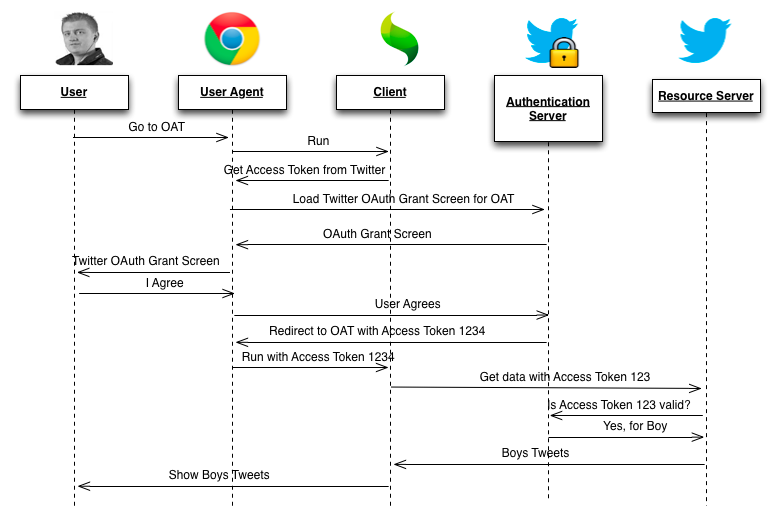
\includegraphics[width=1\textwidth]{images/oauth2.png}
			\caption{http://www.ibuildings.nl/blog/2013/03/secure-your-rest-api-oauth2-implicit-grant}
		\end{figure}

	\end{frame}

	\begin{frame}
		\frametitle{Autres améliorations}
		\begin{itemize}
			\item Performances :
				\begin{itemize}
					\item Amélioration des requêtes SQL ;
					\item Déléguer les requêtes à la base de données (fonction SQL) ;
					\item Changer de type de base de données (Neo4j ou PostgreSQL).
				\end{itemize}
			\item Séparation des services :
				\begin{itemize}
					\item Machines physiques ;
					\item Machines virtuelles.
				\end{itemize}
			\item Fonctionnalités :
				\begin{itemize}
					\item Cases maritimes ;
					\item Proposition de parties.
				\end{itemize}
		\end{itemize}
	\end{frame}

\subsection{Client}
	\begin{frame}
		\frametitle{Client}
		\begin{itemize}
			\item Amélioration de l'interface graphique ;
			\item Carte plus générique ;
			\item Refactor de la communication avec l'API ;
			\item Sérialisation / désérialisation des modèles grâce au JSON.
		\end{itemize}
	\end{frame}
